\documentclass[11pt]{article}
\usepackage[utf8]{inputenc}
\usepackage[portuges]{babel}
\usepackage{a4wide}
\usepackage{setspace}
\usepackage{graphicx}
\usepackage{verbatim}
\usepackage{fancyvrb}
\usepackage{hyperref}

\newcommand{\paragraphnl}[1]{\paragraph{#1}\mbox{}\\}

\DefineVerbatimEnvironment
{MyVerbatim}{Verbatim}
{gobble=0,frame=single}
\fvset{fontsize=\normalsize}

\DefineVerbatimEnvironment
{MyVerbatims}{Verbatim}
{gobble=0,frame=single}
\fvset{fontsize=\scriptsize}

\usepackage{listings}
\usepackage{color}

\definecolor{dkgreen}{rgb}{0,0.6,0}
\definecolor{gray}{rgb}{0.5,0.5,0.5}
\definecolor{mauve}{rgb}{0.58,0,0.82}

\lstset{frame=tb,
  language=Java,
  aboveskip=3mm,
  belowskip=3mm,
  showstringspaces=false,
  columns=flexible,
  basicstyle={\small\ttfamily},
  numbers=none,
  numberstyle=\tiny\color{gray},
  keywordstyle=\color{blue},
  commentstyle=\color{dkgreen},
  stringstyle=\color{mauve},
  breaklines=true,
  breakatwhitespace=true,
  tabsize=3
}

\renewcommand\lstlistingname{Exemplo}



\begin{document}

\begin{titlepage}
\onehalfspacing

\newcommand{\HRule}{\rule{\linewidth}{0.5mm}} % Defines a new command for the horizontal lines, change thickness here

\center % Center everything on the page

%----------------------------------------------------------------------------------------
%    HEADING SECTIONS
%----------------------------------------------------------------------------------------

\textsc{\LARGE Universidade do Minho}\\[1.5cm] % Name of your university/college
\textsc{\Large Mestrado em Engenharia Informática}\\[0.5cm] % Major heading such as course name
\textsc{\large Arquiteturas Aplicacionais}\\[0.5cm] % Minor heading such as course title
\textsc{Ano lectivo 2014/2015}\\[0.5cm]

%----------------------------------------------------------------------------------------
%    TITLE SECTION
%----------------------------------------------------------------------------------------

\HRule \\[0.4cm]
\textsc{\Large Trabalho Prático}\\[0.4cm] % Title of your document
\textsc{ \large Design Patterns}\\[0.4cm] % Title of your document
\HRule \\[1.5cm]

%----------------------------------------------------------------------------------------
%    AUTHOR SECTION
%----------------------------------------------------------------------------------------

\textsc{\large Autores:}\\
{
José Morgado (pg27759) \\
Luís Miguel Pinto (pg27756) \\
Pedro Carneiro (pg25324)
}\\[1cm] % Your name

%----------------------------------------------------------------------------------------
%    DATE SECTION
%----------------------------------------------------------------------------------------

Braga, {\large \today}\\[1cm] % Date, change the \today to a set date if you want to be precise

%----------------------------------------------------------------------------------------
%    LOGO SECTION
%----------------------------------------------------------------------------------------


\includegraphics[scale=0.7]{img/escola-eng.png}\\[0cm] % Include a department/university logo - this will require the graphicx package

%----------------------------------------------------------------------------------------

\vfill % Fill the rest of the page with whitespace

\end{titlepage}


\begin{abstract}
Neste trabalho serão identificadas e analisadas \textit{frameworks} respeitantes a cada uma das três camadas (dados, lógica e apresentação) do modelo de três camadas.

A intenção passa por escolher, para cada uma das camadas referidas anteriormente, a que mais se adequa aos interesses de um programador que pretenda desenvolver uma aplicação.
\end{abstract}


\newpage
\tableofcontents

\newpage
\section{Introdução}


\newpage
\section{Patterns de Criação}

\subsection{Singleton}


Este \textit{pattern} é utilizado quando se pretende a existência de apenas uma instância de uma classe. Para uma classe ser \textit{singleton} deve garantir-se que há apenas uma instância e um ponto de acesso à mesma.

\begin{figure}[!h]
\centering
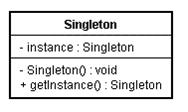
\includegraphics[scale=.9]{img/singleton-diagrama}
\caption{Diagrama de classe}
\end{figure}

No diagrama de classe apresentado anteriormente existe um atributo \textit{singleton} que é do tipo da própria classe. Nos métodos da classe podemos verificar a presença do construtor de classe, \textit{Singleton()}, que é privado. Ora, para que a classe seja instanciada é necessário utilizar o método estático \textit{getInstance()}, assim pode ser acedido por qualquer outra classe.

\begin{lstlisting}[caption=Solução de implementação]
public class MyClass {
  private static MyClass instance = null;

  private MyClass() {
  }

  public static MyClass getInstance() {
    if(instance==null) {
      instance = new MyClass();
    }
    return MyClass.instance;
  }
}
\end{lstlisting}

Com a implementação anterior assegurasse que ao tentar-se criar duas instâncias da mesma classe isso não é possível, pois o atributo \textit{instance} já não está a \textit{null}.

\paragraph{Vantagens}

É um \textit{Pattern} simples e é utilizado quando se pretende ter um acesso único e global para organizar os recursos.

\paragraph{Desvantagens}

A utilização exagerada deste \textit{pattern} pode provocar depedências muito fortes entre os objetos e dificultar alterações de configurações futuras.

\subsection{Prototype}

\subsubsection{Objetivo}

Especificar tipos de objetos usando uma instância prototípica a partir da qual serão criadas cópias da mesma.

\subsubsection{Motivação}

Considere-se uma framework para criação de editores gráficos de partituras:

\centerline{\includegraphics[scale=.7]{img/prototype/motivation.png}}

A classe GraphicTool necessita de componentes gráficos, como por exemplo notas musicais. Estas têm diversas variantes pelo que criar uma subclasse para cada uma pode ser impraticável. Nestes caso, uma alternativa mais adequada será obter novas instâncias da mesma classe a partir de um método Clone() e inicializá-las com diferentes \textit{bitmaps} e durações.

\subsubsection{Aplicação}

Usar quando:
\begin{itemize}
\item as classes a instanciar são especificadas em tempo de execução;
\item se pretende evitar ter uma hierarquia de classes \textit{factory} extensa;
\item instâncias de uma classe apenas podem ter algumas combinações de estado e, por isso, é mais conveniente clonar um protótipo e alterar parte do seu estado do que criar uma nova instância e inicializar todo o seu estado.
\end{itemize}

\subsubsection{Estrutura}

\centerline{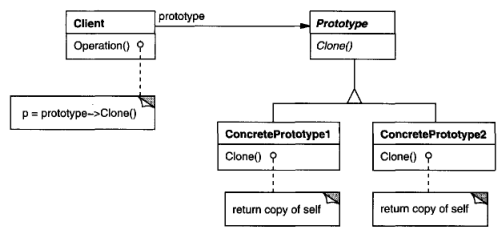
\includegraphics[scale=.7]{img/prototype/structure.png}}

\subsubsection{Participantes}
\begin{itemize}
\item Prototype (Graphic), declara uma interface para criar clones
\item ConcretePrototype (Staff, WholeNote, HalfNote), implementa o método de clonagem
\item Client (GraphicTool), cria novos objetos a partir do protótipo
\end{itemize}

\subsubsection{Colaborações}

Um cliente solicita a um protótipo cópias do mesmo.

\subsubsection{Consequências}
\begin{itemize}
\item Permite incorporar facilmente novas classes concretas de um produto num sistema de uma forma mais flexível relativamente aos restantes padrões de criação porque o cliente pode adicionar e remover protótipos em tempo de execução.
\item Permite reduzir significativamente o número de classes que um sistema necessita.
\end{itemize}

\subsubsection{Implementação}
\begin{itemize}
\item Quando o número de protótipos é dinâmico devemos considerar a utilização de um gestor de protótipos a partir do qual o cliente possa obter e guardar os protótipos.
\item Ao implementar a operação Clone devemos ter em atenção as referências a outros objetos.
\item Se o objeto a clonar não disponibilizar métodos para alterar o seu estado, pode ser necessário adicionar um método Initialize que aceite os parâmetros a inicializar como argumentos.
\end{itemize}

\newpage
\section{Patterns Estruturais}

\subsection{Facade}

O \textit{pattern} Facade esconde toda a complexidade de uma ou mais classes do sistema e fornece uma interface, que o cliente pode aceder  para utilizar o sistema.

Ao se utilizar uma Facade, que implementa uma interface, pretende-se reduzir o nível de complexidade no subsistema, aumentando a facilidade de utilização.\\

\begin{figure}[!h]
\centering
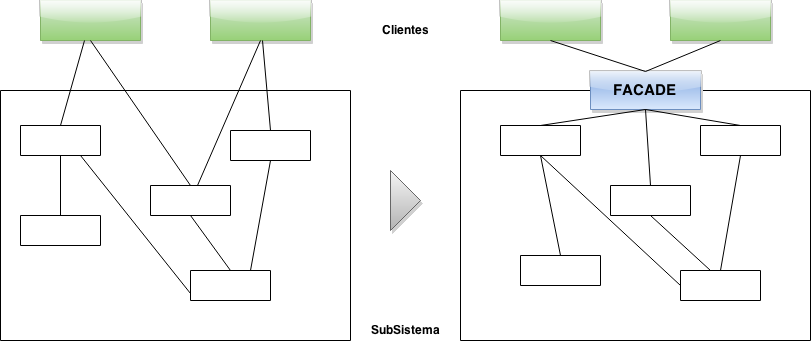
\includegraphics[scale=0.5]{img/facade-estrutura}
\caption{Antes e depois da utilização do Facade}
\end{figure}

Como vemos na figura anterior, este \textit{pattern} é definido através de uma única classe que fornece os métodos necessários ao cliente e envia os pedidos deste às classes do subsistema.\\

\textbf{Aplicação}

Utilizar Facade quando:

\begin{itemize}
  \item Se deseja fornecer uma interface simples para um sistema complexo.
  \item Existe muitas dependências entre clientes e as classes de implementação de uma abstração.
  \item Se pretende ter uma estrutura em camadas no sistema.\\
\end{itemize}

\textbf{Colaboração}

Os clientes comunicam com o subsistema através do envio de pedidos ao Facade, que redireciona os mesmos para as classes apropriadas do subsistema. Ainda que, os clientes que utilizam este \textit{pattern} não tem que aceder aos objetos do seu subsistema diretamente.\\

\textbf{Implementação}

\begin{figure}[!h]
\centering
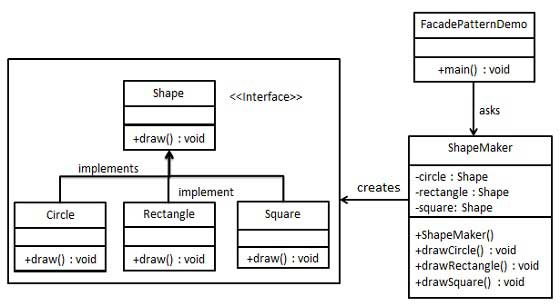
\includegraphics[scale=0.7]{img/facade_diagrama}
\caption{Diagrama de classe}
\end{figure}

Na estrutura seguinte é criada uma interface \textit{Shape} que é implementada por as outras classes do subsistema.

A classe que define o Facade é a \textit{ShapeMaker} e é onde estão definidos os métodos que fornecem contacto aos clientes e as rotinas de gestão dos pedidos para o subsistema.

Por último, a classe \textit{FacadePatternDemo} será o cliente que faz pedidos à classe Facade definida anteriormente.\\

\textbf{Vantagens}

\begin{itemize}
\item A utilização deste \textit{pattern} permite diminuir as ligações entre os clientes e o sistema.
\item Para adicionar novas funcionalidades ao sistema seria necessário alterar apenas o Facade, ao invés de alterar os vários objetos do sistema, sem afetar o cliente.\\
\end{itemize}






\newpage
\subsection{Flyweight}

\subsubsection{Objetivo}

Suportar um grande número de objetos de tamanho reduzido através da partilha de estado entre eles.

\subsubsection{Motivação}

Considere-se por exemplo um editor de texto que necessita de manter a informação aos caracteres existentes num documento. Uma solução seria ter um objeto por caracter, mas isso seria inviável em termos de memória. O padrão Flyweight fornece um mecanismo para contornar esta limitação.

Um flyweight é um objeto partilhado que pode ser utilizado em múltiplos contextos simultaneamente. O conceito chave é a distinção entre estado intrínseco (guardado no flyweight, partilhado) e extrínseco (passado como parâmetro pelos clientes).

Usando este padrão passaríamos a ter a seguinte estrutura:

\centerline{\includegraphics[scale=.7]{img/flyweight/motivation.png}}

Neste caso temos um flyweight para cada letra do alfabeto, responsável por guardar o código do caracter, e quando um cliente necessitar de desenhar uma dada letra recorre ao respetivo flyweight indicando a localização e a fonte pretendidas.

\subsubsection{Aplicação}

Usar quando:
\begin{itemize}
\item a aplicação usa um grande número de objetos;
\item é necessário reduzir a quantidade de objetos em memória;
\item uma grande parte do estado do objeto pode ser partilhada;
\item é possível substituir vários grupos de objetos por um número bem menor de objetos se o estado extrínseco for removido.
\end{itemize}

\subsubsection{Estrutura}

\centerline{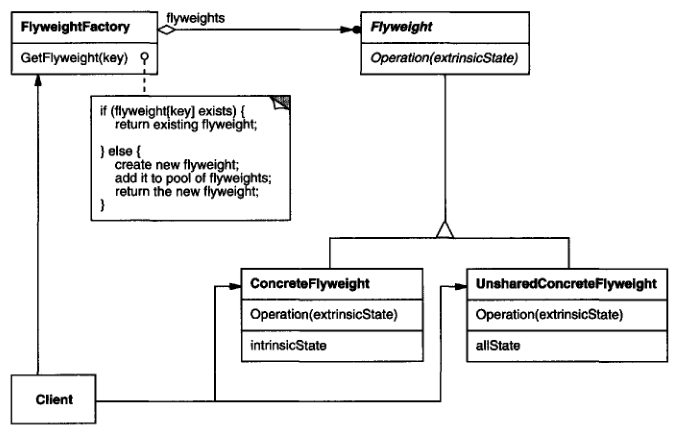
\includegraphics[scale=.7]{img/flyweight/structure1.png}}

O seguinte diagrama demonstra como os flyweights são partilhados:

\centerline{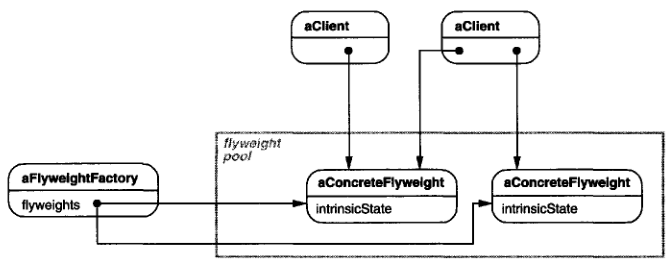
\includegraphics[scale=.7]{img/flyweight/structure2.png}}

\subsubsection{Participantes}
\begin{itemize}
\item Flyweight (Glyph), declara uma interface a partir da qual os flyweights recebem e manipulam o estado extrínseco
\item ConcreteFlyweight (Character), implementa a interface Flyweight e adiciona o estado intrínseco
\item UnsharedConcreteFlyweight (Row, Column), não partilha estado, tipicamente agrega coleções de objetos ConcreteFlyweight
\item FlyweightFactory, cria e gere objetos flyweight
\item Client, mantém as referências para os flyweights e define o seu estado extrínseco
\end{itemize}

\subsubsection{Colaborações}

\begin{itemize}
\item O estado intrínseco é guardado no objeto ConcreteFlyweight e o estado extrínseco é guardado ou calculado por objetos Client.
\item Os clientes não devem criar instâncias ConcreteFlyweight, mas obtê-las a partir de uma FlyweightFactory.
\end{itemize}

\subsubsection{Consequências}
\begin{itemize}
\item As operações associadas à gestão do estado extrínseco podem ter impacto no desempenho.
\item Quantos mais flyweights forem partilhados e quanto maior for o estado partilhado, maior será a poupança de memória.
\item Caso se pretenda combinar este padrão com o padrão Composite, as referências para os pais têm de ser passadas como parte do estado extrínseco.
\end{itemize}

\subsubsection{Implementação}
\begin{itemize}
\item O estado extrínseco deve ser reduzido, caso contrário não será possível tirar partido das vantagens pretendidas.
\item Se o número de flyweights não for fixo e pequeno, pode ser necessário efetuar a gestão dos objetos partilhados por forma a reduzir o impacto ao nível do desempenho e uso de memória.
\end{itemize}


\newpage
\section{Patterns de Comportamento}


\newpage
\section{Conclusão}


\newpage
\section{Referências}

\begin{thebibliography}{99} % Bibliography - this is intentionally simple in this template

\bibitem{Freeman}
Eric Freeman, Elisabeth Robson, Bert Bates, Kathy Sierra. Head First Design Patterns. O'Reilly Media, 2004.

\bibitem{wiki}
http://wiki.portugal-a-programar.pt/dev\_geral:java:padrao\_singleton

\bibitem{devmedia}
http://www.devmedia.com.br/padrao-de-projeto-singleton-em-java/26392

\bibitem{tutorialspoint}
http://www.tutorialspoint.com/design\_pattern/facade\_pattern.htm

\bibitem{Gamma}
Design Patterns: Elements of Reusable Object-Oriented Software, Erich Gamma, Richard Helm, Ralph Johnson, John M. Vlissides, November 1994

\end{thebibliography}


\end{document}
